\section{Supplemental Information}

\subsection{Django overview\label{django-overview}}

\texttt{EspressoDB} utilizes Python's \texttt{Django} Object-Relational
Mapping (ORM) framework. Tables correspond to Python classes, rows
correspond to instances and columns correspond to attributes of the
instances. Thus it is possible to filter for objects by their attributes
or generate summary tables (\texttt{pandas.DataFrame}) within one line
of code. Furthermore, using an ORM allows one to have the same interface
independent of the backend. It is possible to store data in a file based
\texttt{SQLite} solution, or use more scalable options like
\texttt{MySQL} or \texttt{Postgresql}.

\texttt{Django} is part of many open-source projects and thus comes with
extensive documentation. Additionally, \texttt{Django} is scalable,
comes with reliable tests and vast community support which manifests in
the fact that it is commonly used in large scale projects (BitBucket,
Instagram, Mozilla, NASA and many more). One guiding principle of
\texttt{EspressoDB} is to not ``re-invent the wheel'' but instead
leverage the support coming from \texttt{Django}. As a result, one can
easily incorporate many of \texttt{Django}'s extensions and find
solutions to technical questions online.

\subsection{Lattice QCD use case \label{lattice-qcd-use-case}}

LQCD is an inherently a stochastic method of simulating quantum
chromodynamics (QCD) the fundamental theory of nuclear strong
interactions, which is responsible for confining quarks into protons and
neutrons and ultimately, for binding these nucleons into the atomic
nuclei we observe in nature. The application of LQCD to forefront
research applications in nuclear physics is necessary to build a
quantitative connection between our understanding of nuclei and QCD.
This is important as nuclei serve as laboratories and/or detectors for
many experiments aiming to test the limits of the Standard Model of
particle physics in our quest to understand questions such as: Why is
the universe composed of matter and not anti-matter? Does dark matter
interact with regular matter other than gravitationally? What is the
nature of the neutrino and is it related to the observed excess of
matter over anti-matter? See Ref. \cite{Drischler:2019xuo} for a recent
review of the interface of LQCD with our understanding of nuclear
physics.

The application of LQCD to nuclear physics is an exascale challenge. One
of the main reasons these calculations are so expensive is that when
LQCD is applied to systems of one or more nucleons, an exponentially bad
signal-to-noise problem must be overcome. While the optimal strategy for
overcoming this challenge is not yet known, one thing common to all
methods is the need for an exponentially large amount of statistics. As
such, these LQCD computations require the completion of millions of
independent sub-calculations (or tasks), with chained dependencies, in
order to complete a single calculation. These chained tasks write large
amounts of temporary files to the scratch file system which are used as
input for subsequent files, often with multiple input files required for
the later computations. Several such calculations must be performed in
order to extrapolate the results to the physical point, defined as the
limit of zero discretization (the continuum limit), the infinite volume
limit and the limit of physical quark masses which are \emph{a priori}
unknown and so must be determined through this
extrapolation/interpolation procedure. These requirements lead to a very
complex set of computations that must be carried out with great care and
a significant amount of human time and effort to ensure the computing
cycles are used as efficiently as possible.

Compounding these challenges, the new computer Summit, is
\emph{disruptively fast} compared to previous generations of leadership
class computers. Full machine-to-machine, Summit is approximately 15
times faster than Titan when applied to LQCD applications such as those
carried out by CalLat \cite{Berkowitz:2018gqe}. While this is great for
scientific throughput, it also means the management of the computational
jobs has become unwieldy with the management models typically used for
such computations: Summit churns through the computations so fast, and
produces so much data, it is not possible to keep up with the data
processing and management with our older management tools.

As a concrete example, we consider the nucleon elastic form factor
project being carried out by CalLat \cite{incite:2019, incite:2020}.
For each \emph{ensemble} of gauge configurations used (one choice of
input parameters) the computation requires the following dependent
steps:

\begin{enumerate}
\def\labelenumi{\arabic{enumi}.}
\tightlist
\item
  For each gauge configuration (of O(1000)) in an ensemble (of O(20)),
  make several quark sources (grouped in batches of 8);
\item
  For each source, create a quark propagator;
\item
  For each quark propagator:

  \begin{enumerate}
  \def\labelenumii{\arabic{enumii}.}
  \tightlist
  \item
    Create a proton correlation function to determine the proton mass;
  \item
    Create O(10) proton \emph{sequential} sinks at different separation
    times (times 4 for different spin and flavor combinations);
  \end{enumerate}
\item
  For each time-separation, group the 8 \emph{sequential} sinks from the
  8 propagators into a single \emph{coherent sequential} sink
  \cite{Bratt:2010jn};
\item
  For each time-separation, Solve a \emph{sequential} propagator from
  the \emph{coherent sequential} sink;
\item
  For each time-separation, tie each of the original 8 propagators with
  the sequential propagator to construct a 4-dimensional (4D)
  \emph{formfactor} correlation function;
\item
  Process the data to prepare it for analysis and the extraction of
  physics.
\item
  Repeat for multiple source sets (of 8) if more statistics are
  required.
\end{enumerate}

Each of the steps above leads to the generation of many large
(multi-gigabyte) data files, most of which are not saved.
\texttt{LatteDB} is used to track the status of these data files to know
if they need to be created or if the next step can proceed. The final
data production step, 6, leads to our final data file that need further
processing prior to our final analysis and saving of the files.

Inheriting the functionality of \texttt{EspressoDB}, \texttt{LatteDB}
has the flexibility to faithfully reproduce a one-to-one mapping between
the above computational workflow to database tables. For example, in
step 1, the table of gauge configurations is defined such that every row
in the table specifies a single gauge configuration. This reflects how
on disk, we have thousands of files, each containing a snapshot of the
QCD vacuum, and as such, every file, and every subsequent file as a
result of the gauge configuration (\emph{e.g.} propagators or
correlation functions in steps 2 through 6) can also be tracked
individually. However, at the end of the calculation, an observable is
only well defined with an ensemble of gauge configurations.
\texttt{LatteDB} allows one to define an ensemble table, with a
\texttt{Django\ ManyToMany} data type which may be interpreted as a
single column containing a list of references (foreign keys) to the
table of gauge configurations. In \texttt{SQL}, a list of foreign keys
is not a fundamental data type that is supported, and is only made
possible with \texttt{Django}. However, even with \texttt{Django},
unique constraints can not be implemented on such a column. With
\texttt{LatteDB}, we make it possible to define a unique constraint,
which for this example, prohibits the user from inserting the exact same
list of gauge configurations in the ensemble table more than once. Users
are encouraged to consult the documentation of \texttt{EspressoDB} and
examples in \texttt{LatteDB} for more information.

Additionally, \texttt{LatteDB} is also tremendously useful for managing
the data processing steps (step 7) which proceed as:

7a. For each configuration, for each time separation, for each of the 8
sources, \emph{time slice} the 4D data formfactor files to only the time
slices containing relevant data; 7b. For each configuration, for each
time separation, for each source set, average the 8 formfactor\_tsliced
files to a source averaged file. 7c. When all configurations are
complete, concatenate these files together. 7d. As needed, Fourier
Transform these files to project the formfactors onto definite momentum
transfers. 7e. Analyze the correlation functions to extract the relevant
physics.

In Figure 1, we show an example \texttt{LatteDB} Table from step 7b. The
user is able to filter on each column to very quickly assess the
production status (green means the tsliced\_source\_averaged file
exists, red means it is missing) and decide what configurations in what
ensembles need to be managed in production.

More importantly, our production scripts interact with \texttt{LatteDB},
therefore even without the visualization, the scripts will only generate
work that \texttt{LatteDB} records as missing. This interaction with
\texttt{LatteDB} significantly reduces the amount of human time required
to manage the computations. We are actively constructing routines to
also store the final data files to tape, the status of which is stored
in a related \texttt{LatteDB} table. Thus, the user can query the
database instead of the file system for the existence of data files,
significantly reducing the load on the file system as well.
Examples of interacting with \texttt{LatteDB} can be found in
our management repository for these INCITE projects
\url{https://github.com/callat-qcd/nucleon_elastic_FF}.
The scripts for interacting with \texttt{LatteDB} are in the \texttt{scripts} folder and containt \texttt{lattedb} in the name.
Other examples can be found in the \texttt{notebooks} folder in
\texttt{LatteDB}. These scripts will be updated regularly to encompass
more and more utilities from \texttt{EspressoDB} providing a complete
working example.

\begin{figure}
\centering
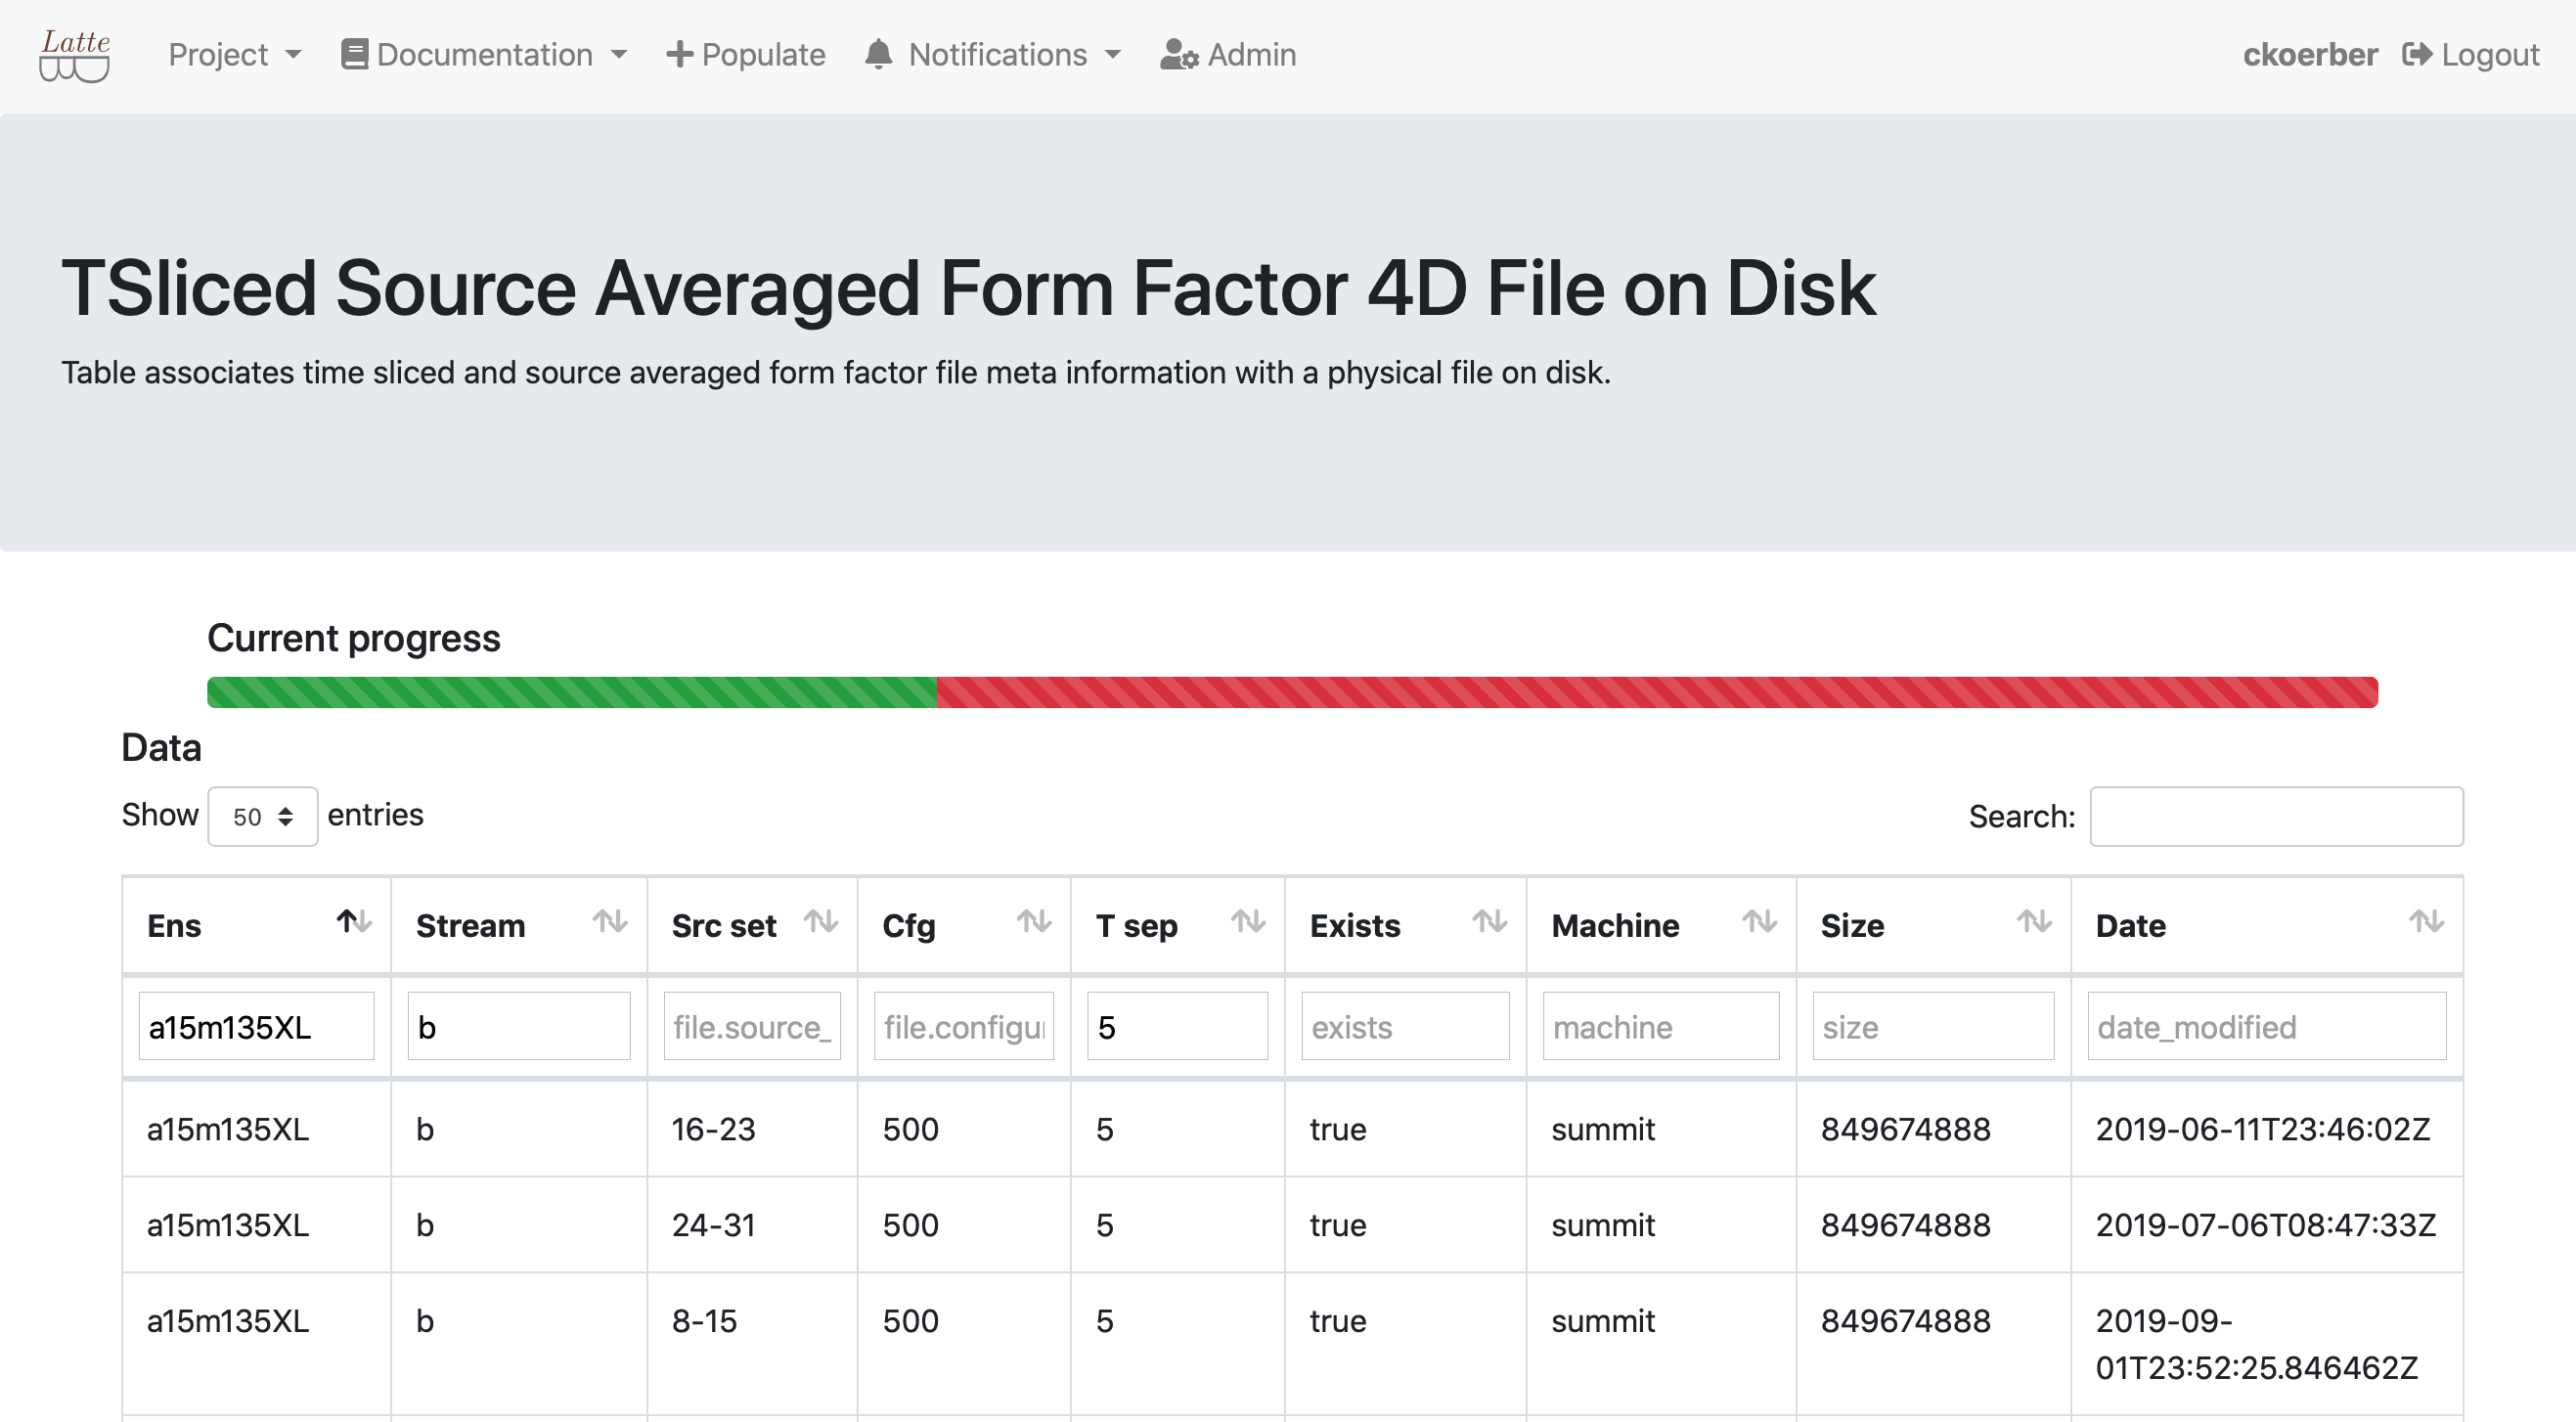
\includegraphics{../_static/lattedb-example.png}
\caption{Example table view of file status with column specific filters
and dynamic progress bar.}
\end{figure}

Other features that can be implemented is the storing of the data files
in \texttt{LatteDB} as well as storing the analysis of the data files.
This allows for communal data analysis within a collaboration with a
centralized location for results, making it easier to combine results
from different members and reduce redundant work. Depending upon the
success and popularity of \texttt{EspressoDB}, it may be worth exploring
whether OLCF (or other LCF) would be willing to allow users to host
databases locally on the machines such that the compute nodes could
interact with the database allowing users to minimize the number of
small input files that are typically written to the file system as well.
In our case, each separate task requires an input file and typically
generates two or three small output files, rapidly polluting the file
system with millions of small files. \texttt{EspressoDB} will minimally
allow users to \emph{clean up} these small files and store the relevant
log and output information in the database.
